\documentclass{article}

\usepackage[english]{babel}

\usepackage[letterpaper,top=1cm,bottom=2cm,left=1.5cm,right=1.5cm,marginparwidth=1.75cm]{geometry}

\usepackage{array}
\usepackage{colortbl}
\usepackage{amsmath}
\usepackage{graphicx}
\usepackage[table,xcdraw]{xcolor}
\usepackage{multicol} % Для двух колонок
\usepackage{titlesec} % Для изменения стиля заголовков
\usepackage{indentfirst}
\usepackage[colorlinks=true, allcolors=blue]{hyperref}
\renewcommand{\thesection}{\Roman{section}} 

\title{\textbf{Desktop Application for Processing 
Text Obtained by Nbconvert and Containing Latex Formulas}}
\author{Khorasandzhyan Levon\\Faculty of Computer Science\\Department of Software Engineering\\National Research University Higher School of Economics\\lakhorasandzhyan@edu.hse.ru}

\begin{document}
\date{}
\maketitle

\begin{multicols}{2}

\textbf{
Abstract — this project proposal presents the development of a desktop application for processing text extracted from Jupyter Notebooks via Nbconvert, particularly focusing on documents containing LaTeX formulas. The project's primary goal is to provide users with a tool that allows selective conversion of Jupyter Notebook content into LaTeX format while ensuring the correct handling of mathematical expressions. At the moment, the application is built using Python with the Tkinter library and features a graphical user interface to preview and configure conversion settings. The anticipated outcome of this project is a functional and user-friendly application that allows people to automatically convert Jupyter Notebooks to LaTeX file format. The target audience that will use the described application consists of researchers, educators, and students.
}

\textbf{Key words — \textit{Jupyter Notebook, LaTeX, Python, Tkinter, Nbconvert, conversion, file}}

\section{Introduction}
The research focuses on automating the conversion of Jupyter Notebooks [1] to the LaTeX [2] format for academic and technical documentation. This area is essential for students, teachers, research fellows, scientists, and data analysts who work with computational notebooks containing mathematical expressions and data analysis.

The problem addressed is the inefficiency and complexity of manually converting Jupyter Notebooks into structured LaTeX documents. This process is time-consuming and prone to formatting errors, especially when handling mathematical equations and large data sets. Automating this task improves productivity and ensures consistent document formatting.

To solve this problem, a desktop application written in Python programming language [3] will be developed to allow users to selectively convert Jupyter Notebook content to LaTeX format while preserving equations and formatting. Graphical user interface will be created using Tkinter library [4][5].

This research builds on existing work related to Jupyter Notebook conversion tools, including Nbconvert, Vertopal, and Ploomber Cloud, analyzing their limitations and enhancing usability.

The proposed approach differs by providing an interactive, user-friendly interface with the ability to preview, customize, and filter notebook content before conversion, improving flexibility and accuracy.

The expected result is a functional desktop application that simplifies the conversion process, improves workflow efficiency, and ensures the generation of high-quality LaTeX documents.

This paper is structured as follows: Section 1 introduces the research area, defining key problems and objectives. Section 2 reviews related work and the theoretical framework. Section 3 outlines the methodology and approaches used to develop the proposed solution. Section 4 analyzes the results and their implications, while Section 5 concludes the paper and explores directions for future research.

\section{Literature review}
One of the main challenges in converting Jupyter Notebooks to LaTeX is preserving formatting, mathematical expressions, and structured content. Several tools exist to address this issue, each with its pros and cons.

Nbconvert [6] is a widely used command line utility that allows users to convert Jupyter Notebooks into various formats, including LaTeX, PDF, and HTML. It supports exporting equations written in Markdown or code cells. However, its usability is limited as it requires command line interaction and manual configuration of templates, making it less accessible to non-technical users.

Vertopal [7] is an online conversion service that simplifies the process by allowing users to upload files and receive output in many different formats, including LaTeX. While convenient, this tool lacks advanced customization options and struggles with complex Jupyter Notebook structures, particularly when handling large data sets or intricate mathematical expressions.

Ploomber Cloud [8] extends notebook transformation capabilities by integrating cloud execution, allowing users to pre-process and execute notebooks before exporting them. This is useful for automated workflows, but introduces a dependency on cloud infrastructure, which may not be ideal for users who prioritize the security of local data.

These existing solutions provide valuable functionality but fall short in offering an intuitive, user-controlled process for selective content conversion. My approach advances these tools by integrating an interactive desktop interface, enabling users to preview and selectively convert notebook sections, including cells with text, code and output, while ensuring accurate LaTeX formatting.

A critical limitation of existing solutions is the lack of fine-grained control over which Jupyter Notebook elements are included in the final tex-document. Most tools perform full document conversion, requiring manual post-processing to remove unwanted content. It's enormously wastes human's time on routine duties.

Research on user-controlled document customization highlights the importance of being able to selectively extract content to maintain document clarity and relevance. While some tools, like Nbconvert, offer filtering options via metadata tags, they require predefined configurations and command line execution, reducing accessibility.

My approach improves upon these methods by providing a graphical interface where users can interactively select specific cells for conversion. This feature provides flexibility, allowing users to include only relevant content without modifying the original Jupyter Notebook structure.

Accurate representation of mathematical expressions and formulas is one of the key requirements when exporting computational notebooks to LaTeX. Inconsistencies in equation formatting can lead to readability issues and hinder the reproducibility of research findings.

To summarize the analysis, let's draw some conclusions using the comparison table below:
\begin{center}
    \renewcommand{\arraystretch}{1.2}
    \setlength{\arrayrulewidth}{0.3mm}
    \setlength{\tabcolsep}{3pt}
    \resizebox{\columnwidth}{!}{
        \begin{tabular}{|p{3.8cm}|c|c|c|c|}
            \hline
            \rowcolor[gray]{0.9} \textbf{\large Criterion} & \textbf{My App} & \textbf{Nbconvert} & \textbf{Vertopal} & \textbf{Ploomber} \\
            \hline
            \large Document\newline Structure\newline Customization & \cellcolor[HTML]{f8fff6} + & \cellcolor[HTML]{fff1f1} - & \cellcolor[HTML]{fff1f1} - & \cellcolor[HTML]{fff1f1} - \\
            \hline
            \large Content Customization for tex Output & \cellcolor[HTML]{f8fff6} + & \cellcolor[HTML]{fff1f1} - & \cellcolor[HTML]{fff1f1} - & \cellcolor[HTML]{fff1f1} - \\
            \hline
            \large Mathematical\newline Expressions\newline Support & \cellcolor[HTML]{f8fff6} + & \cellcolor[HTML]{fff8e6} +/- & \cellcolor[HTML]{fff8e6} +/- & \cellcolor[HTML]{fff8e6} +/- \\
            \hline
            \large Cyrillic\newline Characters\newline Support & \cellcolor[HTML]{f8fff6} + & \cellcolor[HTML]{fff1f1} - & \cellcolor[HTML]{fff1f1} - & \cellcolor[HTML]{fff1f1} - \\
            \hline
            \large Data\newline Visualization\newline Support & \cellcolor[HTML]{f8fff6} + & \cellcolor[HTML]{fff1f1} - & \cellcolor[HTML]{f8fff6} + & \cellcolor[HTML]{fff1f1} - \\
            \hline
            \large Preview Before\newline Download & \cellcolor[HTML]{f8fff6} + & \cellcolor[HTML]{fff1f1} - & \cellcolor[HTML]{f8fff6} + & \cellcolor[HTML]{fff1f1} - \\
            \hline
            \large Local Data\newline Processing & \cellcolor[HTML]{f8fff6} + & \cellcolor[HTML]{f8fff6} + & \cellcolor[HTML]{fff1f1} - & \cellcolor[HTML]{fff1f1} - \\
            \hline
            \large Folder/Archive\newline Upload & \cellcolor[HTML]{f8fff6} + & \cellcolor[HTML]{fff1f1} - & \cellcolor[HTML]{fff1f1} - & \cellcolor[HTML]{fff1f1} - \\
            \hline
            \large No Ads & \cellcolor[HTML]{f8fff6} + & \cellcolor[HTML]{f8fff6} + & \cellcolor[HTML]{fff1f1} - & \cellcolor[HTML]{fff1f1} - \\
            \hline
        \end{tabular}
    }
\end{center}

\section{Methods}
This study examines the effectiveness of a desktop application under development for converting Jupyter notebooks to LaTeX, allowing users to self-select the content to be exported. The main hypothesis is that a flexible, user-controlled process for interacting with the Jupyter Notebook source file will improve the efficiency and accuracy of user queries compared to existing automated or command-line-based solutions. Additionally, it is hypothesized that providing a preview feature will improve the user's understanding of what they expect from the final document.

The application follows a structured step-by-step approach to document conversion, using a graphical user interface (GUI) to facilitate user interaction. The system expects Jupyter notebooks to contain a mixture of text, code, and output cells, including mathematical equations and formulas, and that users require control over which sections to include in the final LaTeX document. It is also assumed that users may not have previous experience with LaTeX or command-line tools, requiring the GUI to be intuitive.

It was decided to use Python as the programming language to be used. The decisive factors that I relied on when choosing it were the following: brevity, high level of the language, a large number of implemented libraries. In addition, Python also provides a cross-platform event-oriented graphical library Tkinter. It is easy to use and is also included in the standard Python library. When interacting directly with the original Jupyter Notebook, the notebook processing libraries nbconvert and nbformat [9] are used. They are used to read, present, analyze and export Jupyter notebooks to the requested format. All the programs and tools used are open source and widely distributed. The system design follows the Model-View-Controller (MVC) [10] architectural pattern to ensure modularity and ease of maintenance. The "Model" handles the logic of data processing and transformation, the "View" represents the graphical interface, and the "Controller" manages user input and interaction. Let's consider the principle of using this pattern in practice. The starting point is in the \texttt{main.py} file in the main \texttt{src} package. In this file, the application is initialized and launched via the \texttt{FormuLabApplication} class. In the future, the object of this class, passed to various methods of the \texttt{MVC} package, will act as the application navigator (implementing transitions between different windows). During the initial launch, after the user interacts with the program interface, the functions of the \texttt{MainMenuView} class, bound to the corresponding buttons, are subsequently triggered. The received user request is redirected to the \texttt{MainMenuController} class. Then the controller passes the received request to the \texttt{MainMenuModel} model and waits for the received data for further interaction with the user. The interaction of the \texttt{CellSelectorView}, \texttt{CellSelectorModel} and \texttt{CellSelectorController} classes occurs in a similar way.

The study measures the efficiency and accuracy of the conversion process according to the following criteria:
Processing time - a comparison of the time required to convert a Jupyter notebook using the developed application compared to the previously mentioned existing tools;
Formatting accuracy - an assessment of the correctness of the display of mathematical expressions and formulas in the resulting file.

To test the effectiveness of the developed tool, a comparative analysis is performed using test cases with Jupyter notebooks containing different content structures. The tests are performed manually by simply launching each of the presented applications and then loading the original test file into the system under consideration for analysis. The obtained data in the form of an output tex file are analyzed using both statistical methods and independent human visual analysis of the obtained display of the result in the PDF file format. The LaTeX compiler is used for static analysis. It allows you to automatically check the obtained tex file for syntax errors, as well as obtain a display of the correctly compiled layout in PDF format. When comparing the work of the presented existing solutions, no significant problems with the file processing time were found. Despite this, several errors occurred with the presented display of the obtained tex file. Let us focus on the most key problem - the output of the display of the resulting mathematical expression beyond the boundaries of the sheet visibility area (Fig. 1).\newline

\begin{minipage}[t]{0.9\linewidth}
    \raggedright
    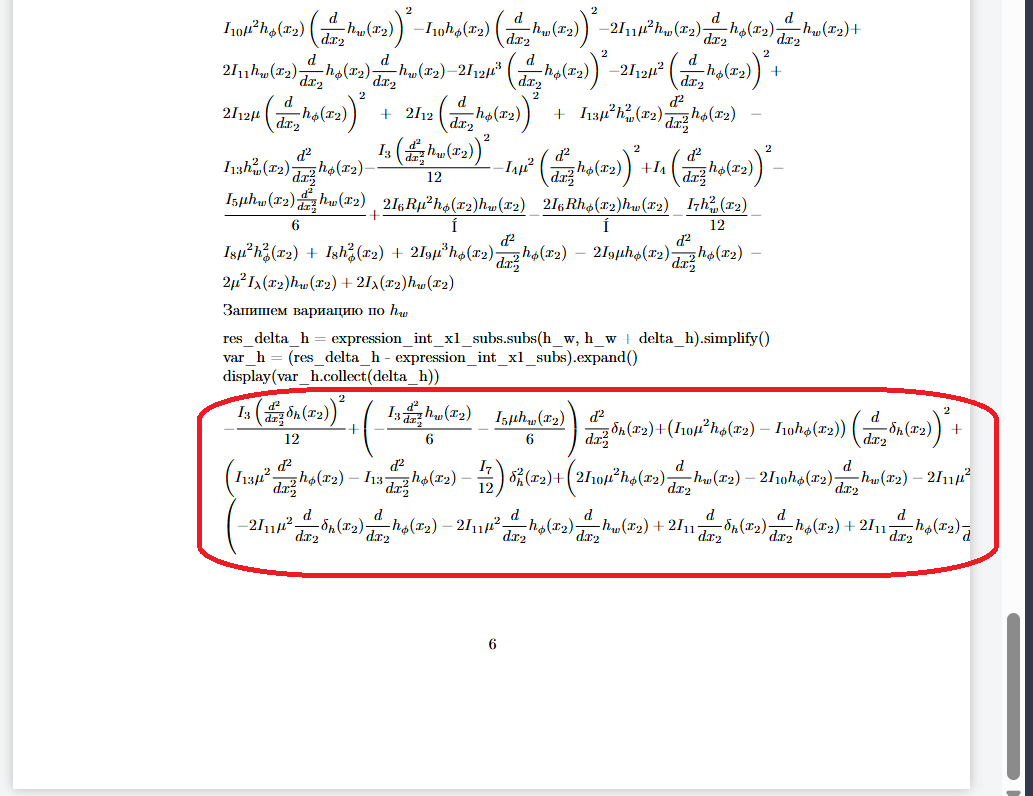
\includegraphics[width=\linewidth, height=0.35\textheight]{fig_1.png}
    \textit{Fig. 1. Mathematical expression exceeding page boundaries\newline}
    \label{fig:math_overflow}
\end{minipage}


The reason for this oversight is that when receiving the display result of the launched code cell, automatic insertion of line breaks was not provided. It was assumed that the output of the launched code cell would be viewed exclusively in the used development environment, which provides horizontal scrolling for too long program output. As a result, the output does not contain line breaks, although in our case with the conversion of Jupyter Notebook to LaTeX format, this is necessary for correct display.

\section{Results}
The developed application successfully allows you to selectively convert Jupyter Notebook content to LaTeX while maintaining the integrity of mathematical formulas. The interface is intuitive, streamlines the conversion process and improves the efficiency of the workflow. The application allows you to fine-tune the content, surpassing existing tools in terms of flexibility. Moreover, in other applications, I encountered the problem of displaying complex mathematical expressions that sometimes did not align perfectly in the final LaTeX output, slightly deviating from the expected results. However, this will be solved by inserting line breaks according to the set limitation of the size of the mathematical formula.

\section{Conclusion}
The developed desktop application efficiently converts Jupyter Notebook content to LaTeX, correctly represents mathematical expressions, and provides customizable LaTeX output. This result is important because it simplifies the document creation process for researchers and educators, saving time and improving formatting accuracy. However, further improvements could be aimed at better handling complex data visualizations to ensure a perfect conversion. Future work could explore adding support for more file formats and integrating additional features such as batch processing for large notebook sets.

\bibliographystyle{alpha}
\scriptsize
\begin{thebibliography}{10}
    \bibitem{notebooks} Kluyver, T., et al. (2016). Jupyter Notebooks - A Publishing Format for Reproducible Computational Workflows. Retrieved February 20, 2025, from \url{https://eprints.soton.ac.uk/403913/}
    \bibitem{latex} Lamport, L. (1994). LaTeX: A Document Preparation System. Retrieved February 20, 2025, from \url{https://archive.org/details/la-te-x-a-document-preparation-system/}
    \bibitem{python} Python Software Foundation. (n.d.). Python Programming Language. Retrieved February 20, 2025, from \url{https://www.python.org}
    \bibitem{tkinter} Lumholt, S., \& van Rossum, G. (n.d.). Tkinter Library Documentation. Retrieved February 20, 2025, from \url{https://docs.python.org/3/library/tkinter.html}
    \bibitem{tkinter2} Lundh, F. (n.d.). An Introduction to Tkinter. Retrieved February 20, 2025, from \url{https://ftp.math.utah.edu/u/ma/hohn/linux/tcl/an-introduction-to-tkinter.pdf}
    \bibitem{nbconvert} Jupyter. (n.d.). Nbconvert Library Documentation. Retrieved February 20, 2025, from \url{https://nbconvert.readthedocs.io/en/stable/}
    \bibitem{vertopal} Vertopal. (n.d.). Online File Converter. Retrieved February 20, 2025, from \url{https://www.vertopal.com}
    \bibitem{ploomber} Ploomber. (n.d.). Ploomber Cloud Documentation. Retrieved February 20, 2025, from \url{https://docs.ploomber.io/en/latest/}
    \bibitem{nbformat} Black Duck Software. (n.d.). Nbformat Library Documentation. Retrieved February 20, 2025, from \url{https://nbformat.readthedocs.io/en/stable/}
    \bibitem{designpatterns} Kamthan, S. (2019). Mastering Python Design Patterns. Retrieved February 20, 2025, from \url{https://www.programmer-books.com/wp-content/uploads/2019/12/Mastering-Python-Design-Patterns.pdf}
\end{thebibliography}

\end{multicols}

\hfill \textbf{Word Count: 1611}

\end{document}